%-------------------------------------------------------------------------
% Design Project Input/Output Module Description
%-------------------------------------------------------------------------

\clearpage
\section{RGB LED Output Module}
\label{sec-output-rgb}

This output module enables your IoT device to display colored light
using an RGB LED (three LEDs in a single housing), where RGB stands for 'red',
'green', and 'blue'. Using the RGB LED, we can generate any color we
desire through color mixing. Do you remember color wheels from
elementary school?

% TODO: add in color table here

A sample circuit and Arduino code is shown below to get you started.
Three leads of the RGB LED are set by digital output Arduino pins
corresponding to 'red', 'green', and 'blue'; the longest lead of the RGB
LED provides power. The example code will set the color of the RGB LED
to violet. After setting up the circuit and programming the Arduino,
check to make sure the RGB LED lights up violet. You can then
experiment with other colors by choosing your own RGB values, and if you
like, you can also try to make the LED blink or change colors in time.

\vspace{0.1in}
\begin{minipage}[t]{0.49\tw}
  \vspace{0pt}

  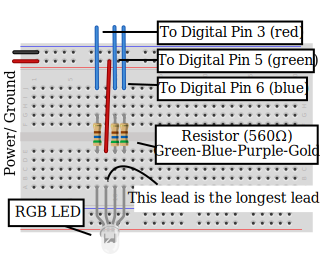
\includegraphics[width=\tw]{output-rgb-annotated.svg.pdf}
\end{minipage}
\hfill
\begin{minipage}[t]{0.49\tw}
  \vspace{0.1in}
  \begin{Verbatim}[gobble=3,fontsize=\small]
    // Choose RGB LED pins (these must be PWM pins)
    // redPin = 3, greenPin = 5, bluePin = 6
    int pin_RGB[] = {3, 5, 6};

    void setup() {
      for (int i = 0; i < 3; i++) {
        pinMode( pin_RGB[i], OUTPUT );
      }
    }

    void loop() {
      // Choose the RGB (red, green, blue) value
      // In this demo, we choose violet.

      byte my_color[] = {23, 0, 22};

      // Iterate through each of the three pins
      // (red, green blue).

      for (int i = 0; i < 3; i++) {

        // Write the analog value to the pin. We
        // use (255 - value) because our RGB LED
        // is common anode, which means the color
        // is fully on when we output
        // analogWrite( pin, 0 ) and fully off when
        // we output analogWrite( pin, 255).

        analogWrite( pin_RGB[i], 255 - my_color[i] );
      }
    }
  \end{Verbatim}
\end{minipage}
\vspace{0.1in}

%Questions:
